\documentclass[a4paper,twoside, openright,12pt]{report}
\usepackage{psfrag,amsbsy,graphics,float}
\usepackage{graphicx, color} %Deleted [dvips] in front of {graphicx, color} for usage also with PDFLaTex
\usepackage[latin1]{inputenc}
\usepackage{verbatim} 
\usepackage{subfig}
\usepackage{amssymb}
\usepackage{amsmath}
\usepackage{verbatimbox}
\usepackage{moreverb}
\usepackage{hyperref}
\hypersetup{
	colorlinks,
	citecolor=black,
	filecolor=black,
	linkcolor=black,
	urlcolor=black
}

%%% Stand 14.09.2007
%%% erstellt von Marion Sobotka
%%% marion.sobotka@tum.de
%%% last changes: 14.01.09


%_______Kopf- und Fußzeile_______________________________________________________
\usepackage{fancyhdr}
\pagestyle{fancy}
%um Kopf- und Fußzeile bei chapter-Seiten zu reaktivieren
\newcommand{\helv}{%
   \fontfamily{phv}\fontseries{a}\fontsize{9}{11}\selectfont}
\fancypagestyle{plain}{	
	\fancyfoot{}% keine Fußzeile
	\fancyhead[RE]{\helv\leftmark}% Rechts auf geraden Seiten=innen; in \leftmark stehen \chapters
	\fancyhead[LO]{\helv\rightmark}% Links auf ungeraden Seiten=außen;in \rightmark stehen \sections
	\fancyhead[RO,LE]{\thepage}}%Rechts auf ungeraden und links auf geraden Seiten
%Kopf- und Fußzeile für alle anderen Seiten
\fancyfoot{}
\fancyhead[RE]{\helv\leftmark}
\fancyhead[LO]{\helv\rightmark}%alt:\fancyhead[LO]{\itshape\rightmark}
\fancyhead[RO,LE]{\thepage}
%________________________________________________________________________________


%_Definieren der Ränder und Längen__________
\setlength{\textwidth}{15cm}
\setlength{\textheight}{22cm}
\setlength{\evensidemargin}{-2mm}
\setlength{\oddsidemargin}{11mm}
\setlength{\headwidth}{15cm}
\setlength{\topmargin}{10mm}
\setlength{\parindent}{0pt} % Kein Einrücken beim Absatz!!
%___________________________________________

%_Hyperref for CC Url__________
\usepackage{hyperref}
%___________________________________________

%_______Titelseite__________________________________________
\begin{document}
\pagestyle{fancy}
\enlargethispage{4.5cm} %Damit das Titelbild weit genug unten ist!
\begin{center}
\phantom{u}
\vspace{0.5cm}
\Huge{\sc Point-cloud Multiple Object Tracking (PMOT)}\\
\vspace{1.5cm}
                                 \large{Software manual

						\vspace{0.4cm}
					PhD. Seongyong Koo\\
						\vspace{0.5cm}

					\vspace{1.5cm}
					Lehrstuhl f\"ur\\
					STEUERUNGS- und REGELUNGSTECHNIK \\
					Technische Universit\"at M\"unchen\\
					\vspace{0.3cm}
					Dynamic Human-Robot-Interaction Group/Prof. Dongheui Lee}
\end{center}
\vspace{5.5cm}
\begin{tabular}{ll}
Beginn: & 01.06.2014  \\
Abgabe: &  31.03.2015 \\
\end{tabular}

%_________Inhaltsverzeichnis__________________________
\tableofcontents 
%_____________________________________________________


\chapter{Introduction}
This document aims at introducing a new open-source software for tracking multiple unknown and random objects from point-cloud video that can be easily captured by low-cost and fast RGB-D camera \footnote[1]{e.g. ASUS Xtion Pro, Microsoft Kinect sensor, and Softkinectic iisu Pro series.}. The product named Point-cloud Multiple Object Tracking (PMOT)\footnote[2]{http://www.hri.ei.tum.de/pmot/} features real-time, model-free, and standalone software by means of using highly trusted and actively developing technologies such as  Robot Operating System (ROS) \footnote[3]{http://www.ros.org/}, point cloud library (PCL)\footnote[4]{http://pointclouds.org/}, and Compute Unified Device Architecture (CUDA)\footnote[5]{https://developer.nvidia.com/cuda-zone}. Especially, this book is a generic user-guide for engineers and researchers who want to utilize the results of PMOT, which are point-level object indexes and object-level 3D poses. To make them easy to understand the software, the following chapters include each content of functionality, installation steps, execution steps, related data set, and reference for source files. 

First of all, this chapter explains the main functionality of PMOT with brief summary of the related scientific papers.
It will give you theoretical background to help your understanding of the software.

\section{Background: Point-cloud object segmentation and tracking}
Point-cloud is a set of 6-dimensional points, each of which contains x,y,z,r,g,b information in the 3D space. In order to identify individual moving objects from a fast RGB-D camera, there have been two different approaches: model-based object tracking and model-free object segmentation. The first approach is mainly for 6D pose estimation of a known single object while the second one is extracting each point-cloud that is involved in each individual object among multiple and unknown objects in the scene point-cloud.
Considering each object segment a representative point, in the second approach, tracking is a problem of constructing temporal associations among multiple object segments between consecutive time frames, which is called multiple object tracking (MOT). Fig. \ref{fig:examples} shows four existing methods for the two tracking approaches. 

\begin{figure}[t]
\centering
	\subfloat[Model-based 3D object tracking in  \cite{Rusu_ICRA2011_PCL}]{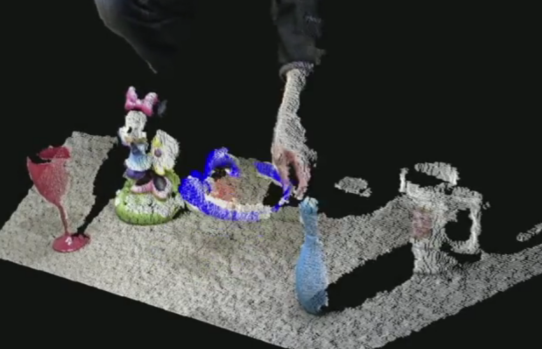
\includegraphics[width=0.45\linewidth]{fig/example_pcltracking.png}%
	\label{fig_first_case}}
	\hfil
	\subfloat[Model-based 3D object tracking in \cite{choi2013rgb}]{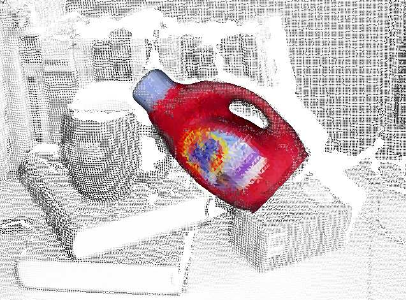
\includegraphics[width=0.45\linewidth]{fig/example_gputracking.png}%
	\label{fig_second_case}}
	\hfil
	\subfloat[Model-free multiple object segmentation and tracking in \cite{papon2013point}]{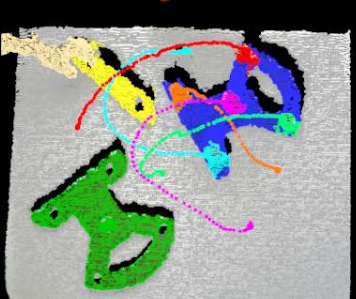
\includegraphics[width=0.45\linewidth]{fig/example_supervoxel.png}%
	\label{fig_second_case}}
	\hfil
	\subfloat[Model-free multiple object segmentation and tracking in  \cite{koo2013multiple}]{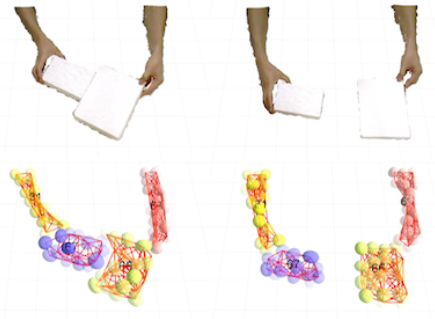
\includegraphics[width=0.45\linewidth]{fig/example_koo.png}%
	\label{fig_second_case}}
	\caption{Existing point-cloud object tracking softwares}
	\label{fig:examples}
\end{figure}

Although the two approaches have been significantly developed in the recent studies \cite{Rusu_ICRA2011_PCL, choi2013rgb, papon2013point, koo2013gmm, koo2013multiple, koo2014incremental, koo2014unsupervised, li2015realtime, papon2015spatially}, they still have unreleased issues that are involved a trade-off with respect to the prior existence of corresponding object models.
The model-based tracking is relatively faster and more precise than model-free tracking, but it requires constructing an accurate object model prior to tracking the specific target, which limits its application domain. On the other hand, the model-free approach allows to track multiple unknown objects without any prior knowledge. However, due to the model-less property, it performs lower tracking performance in not only accuracy but also computation time. 

These difficulties call for a new method that can have advantages of both
approaches, which achieves \textit{accurate} tracking performance for \textit{multiple unknown objects} in \textit{real-time} \textit{without any prior knowledge}.
With this goal in mind, PMOT has been realized as the result of a series of our prior works in \cite{koo2013gmm, koo2013multiple, koo2014incremental, koo2014unsupervised, li2015realtime}. 
The main function of PMOT is processing an input point-cloud and producing information of each individual object at each time step as shown in Fig. \ref{fig:pmot_problem}.
\begin{figure}[t]
	\centering
	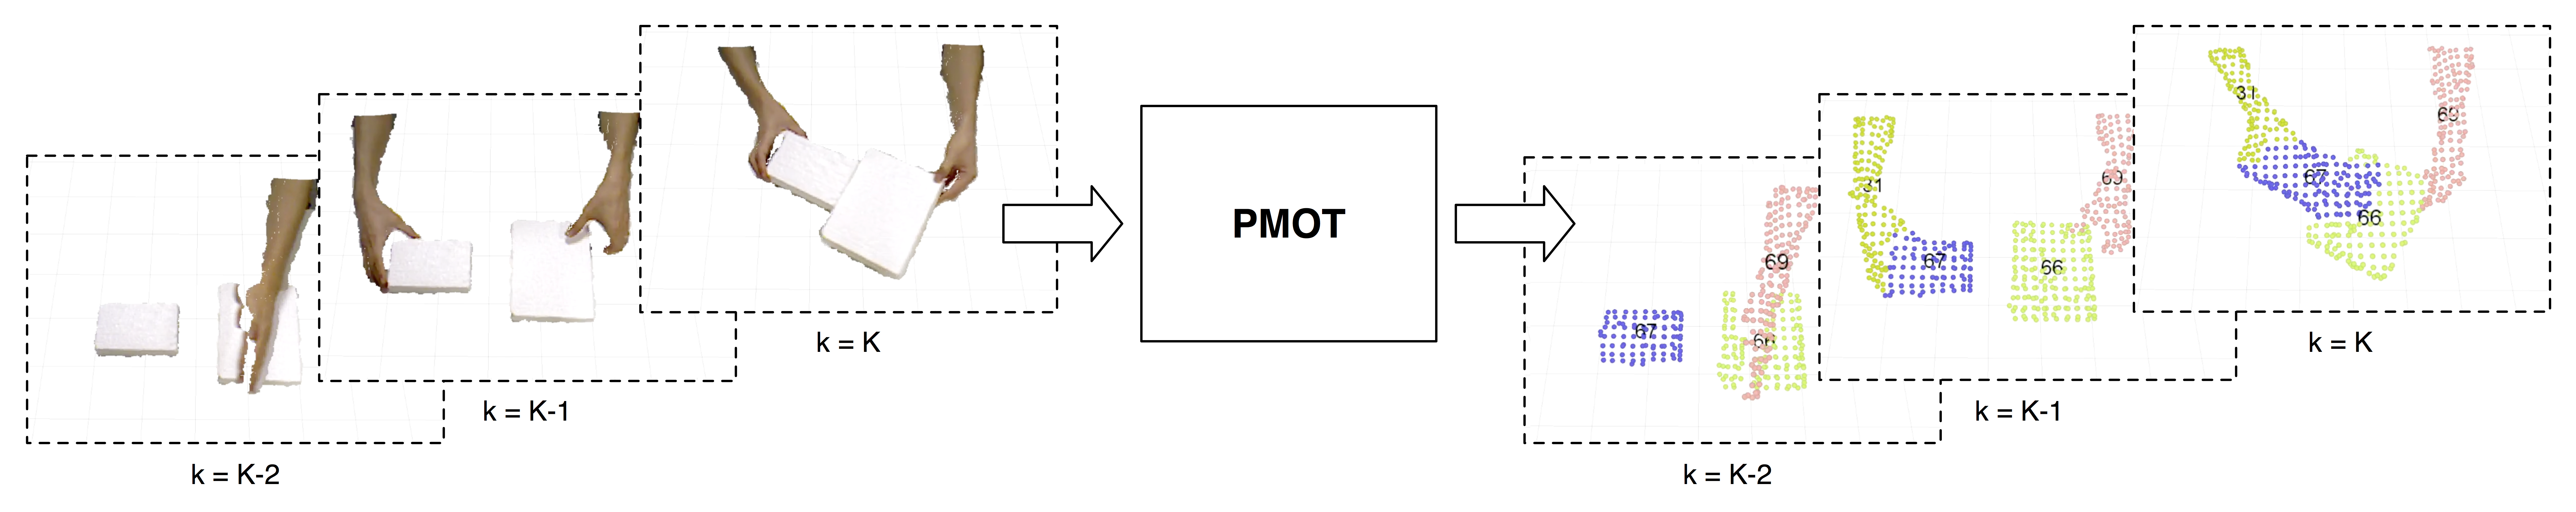
\includegraphics[width=\linewidth]{fig/pmot_problem.png}
	\caption{Input and output of PMOT}
	\label{fig:pmot_problem}
\end{figure}

\section{Simultaneous multiple object segmentation and tracking (SMOST)}

To give you a principle idea behind how PMOT works, this section describes a formal definition of a main problem in PMOT: simultaneous multiple object segmentation and tracking (SMOST).
With the input point-cloud at each time step $t$, ${\bf{P}}_t = \{{\bf{p}}_{1}, ..., {\bf{p}}_{n}\}$, each of which contains the 3-dimensional XYZ position and RGB color of a measured point on the object surface, SMOST estimates object indexes of the point cloud, ${\bf{O}}_t$, and 3D poses and shapes of multiple objects ${\mathcal{X}}_t$ at each time step.
\begin{eqnarray}
SMOST({\bf{P}}_t) \rightarrow \{{\bf{I}}_t, {\mathcal{X}}_t\}	\label{eq:dss_measurement_sko}
\end{eqnarray}
Here, the object indexes, ${\bf{I}}_t = \{I({\bf{p}}_{1}), ..., I({\bf{p}}_{n})\}$ is a set of index variables $I({\bf{p}}_i) \in {\mathbb{I}}$ of each point ${\bf{p}}_i$, which indicates one of the $k$ objects $\mathbb{I}=\{o_1,...,o_k\}$, $o_i \in \mathbb{N}$ where the point is involved.
The second output of SMOST is a set of $k$ constructive object models, ${\mathcal{X}}_t = \{ {\mathcal{X}}_t^{(1)}, ...,  {\mathcal{X}}_t^{(k)} \}$.
Constructive object model of an object $i$, ${\mathcal{X}}_t^{(i)}=\{ {\bf{M}}_t^{(i)}, {\bf{X}}_t^{(i)} \}$, consists of a model point cloud ${\bf{M}}_t^{(i)}$, and 3D pose ${\bf{X}}_t^{(i)}$.

As you see in the Fig. \ref{fig:objectmodel}, input point-cloud ${\bf{P}}_t$ is represented from the world coordinate $W$, while the model point-cloud ${\bf{M}}_t^{(i)}$ is represented from the moving coordinate at each time, $O_t^i$.
\begin{equation}
{\bf{M}}_t^{(i)}= \{{\bf{p}}_{1}, ..., {\bf{p}}_{n_i}\}_{\arrowvert O_t^i}
\end{equation} 
The object pose in the 3D space ${\bf{X}}_t^{(i)}$ is represented as 6-DOF pose in $SE(3)$ group of the object coordinate $O_t^i$ relative to the world coordinate $W$:
\begin{equation}
{\bf{X}}_t^{(i)}= \{x,y,z,roll,pitch,yaw\}_{O_t^i \arrowvert W}
\end{equation} 

\begin{figure}[t]
	\centering
	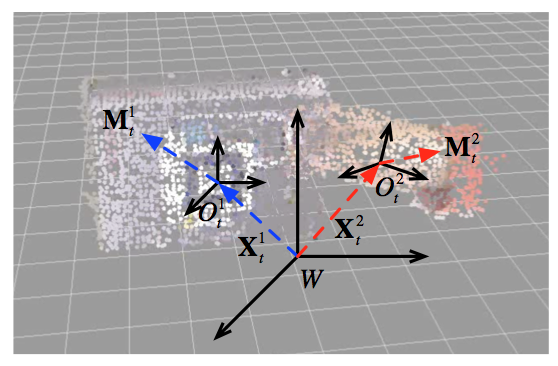
\includegraphics[width=0.5\linewidth]{fig/objectmodel.png}
	\caption{An example of constructive object models and their coordinates}
	\label{fig:objectmodel}
\end{figure}

How does SMOST work? Fig. \ref{fig:concept} shows a block diagram of the SMOST implementation. 
At each time step $t$, the only input is a point-cloud ${\bf{P}}_t$ from a camera. The first step is object segmentation of the point-cloud with previously constructed object models, ${\mathcal{X}}_{t-1}$. Without explicit object models that should be designed from the outside of the program, the object model ${\mathcal{X}}$ is internally constructed at every time step. 
With ${\mathcal{X}}_{t-1}$, the segmentation process is regarded as finding a index function, $I(\cdot)$, to match each point to one of the object indexes. As one of the possible solutions, the function can be defined to find the closest object around each point. 
\begin{equation}
I_t({\bf{p}}_{t})=\underset{j}{\arg\min}\lVert{\bf{p}}_{t}-{\mathcal{X}}_{t-1}^{(j)}\rVert
\end{equation} 

After the segmentation step, the input-point cloud can be grouped according to the object indexes, $\{{\bf{P}}_{t}^{(1)},...,{\bf{P}}_{t}^{(k)}\}$, each of which becomes a new measurement point-cloud for each object. Now the multiple object tracking problem can be converted to a set of separated single object tracking problems. At each $i$ object, the tracking problem consists of two parallel steps: pose estimation and model update. The pose estimation is to update the previous object pose ${\bf{X}}_{t-1}^{(i)}$ with the new measurement ${\bf{P}}_{t}^{(i)}$ and internal object model ${\bf{M}}_{t-1}^{(i)}$ by using a Bayesian Filtering technique \cite{li2015realtime}. In our PMOT, we used GPU-based particle filter which is similar to the method in \cite{choi2013rgb}.
The model update step is incrementally construct a model point-cloud ${\bf{M}}_t^{(i)}$ for each object $i$ with the new measurement ${\bf{P}}_{t}^{(i)}$. In this software, the new model point-cloud is randomly sampled from the old model point-cloud, ${\bf{M}}_{t-1}^{(i)}$, and new measurement point-cloud, ${\bf{P}}_{t}^{(i)}$ with a fixed ratio parameter, which can be defined by a user.
The updated object models, ${\mathcal{X}}_{t}$, are then feedback to the both segmentation and tracking steps in the next time step. 
  
Note that this is a conceptual diagram to represent an overview of data flows and main process blocks, which is not exactly same as source codes of PMOT. More details can be found in our research papers \cite{li2015realtime, koo2014unsupervised, koo2014incremental, koo2013multiple, koo2013imft, koo2013gmm}.

As outputs of PMOT, all information of point-level object indexes ${\bf{I}}_t$ and object-level state data ${\mathcal{X}}_{t}$ can be provided to the user by following the remaining chapters.
 
\begin{figure}[t]
	\centering
	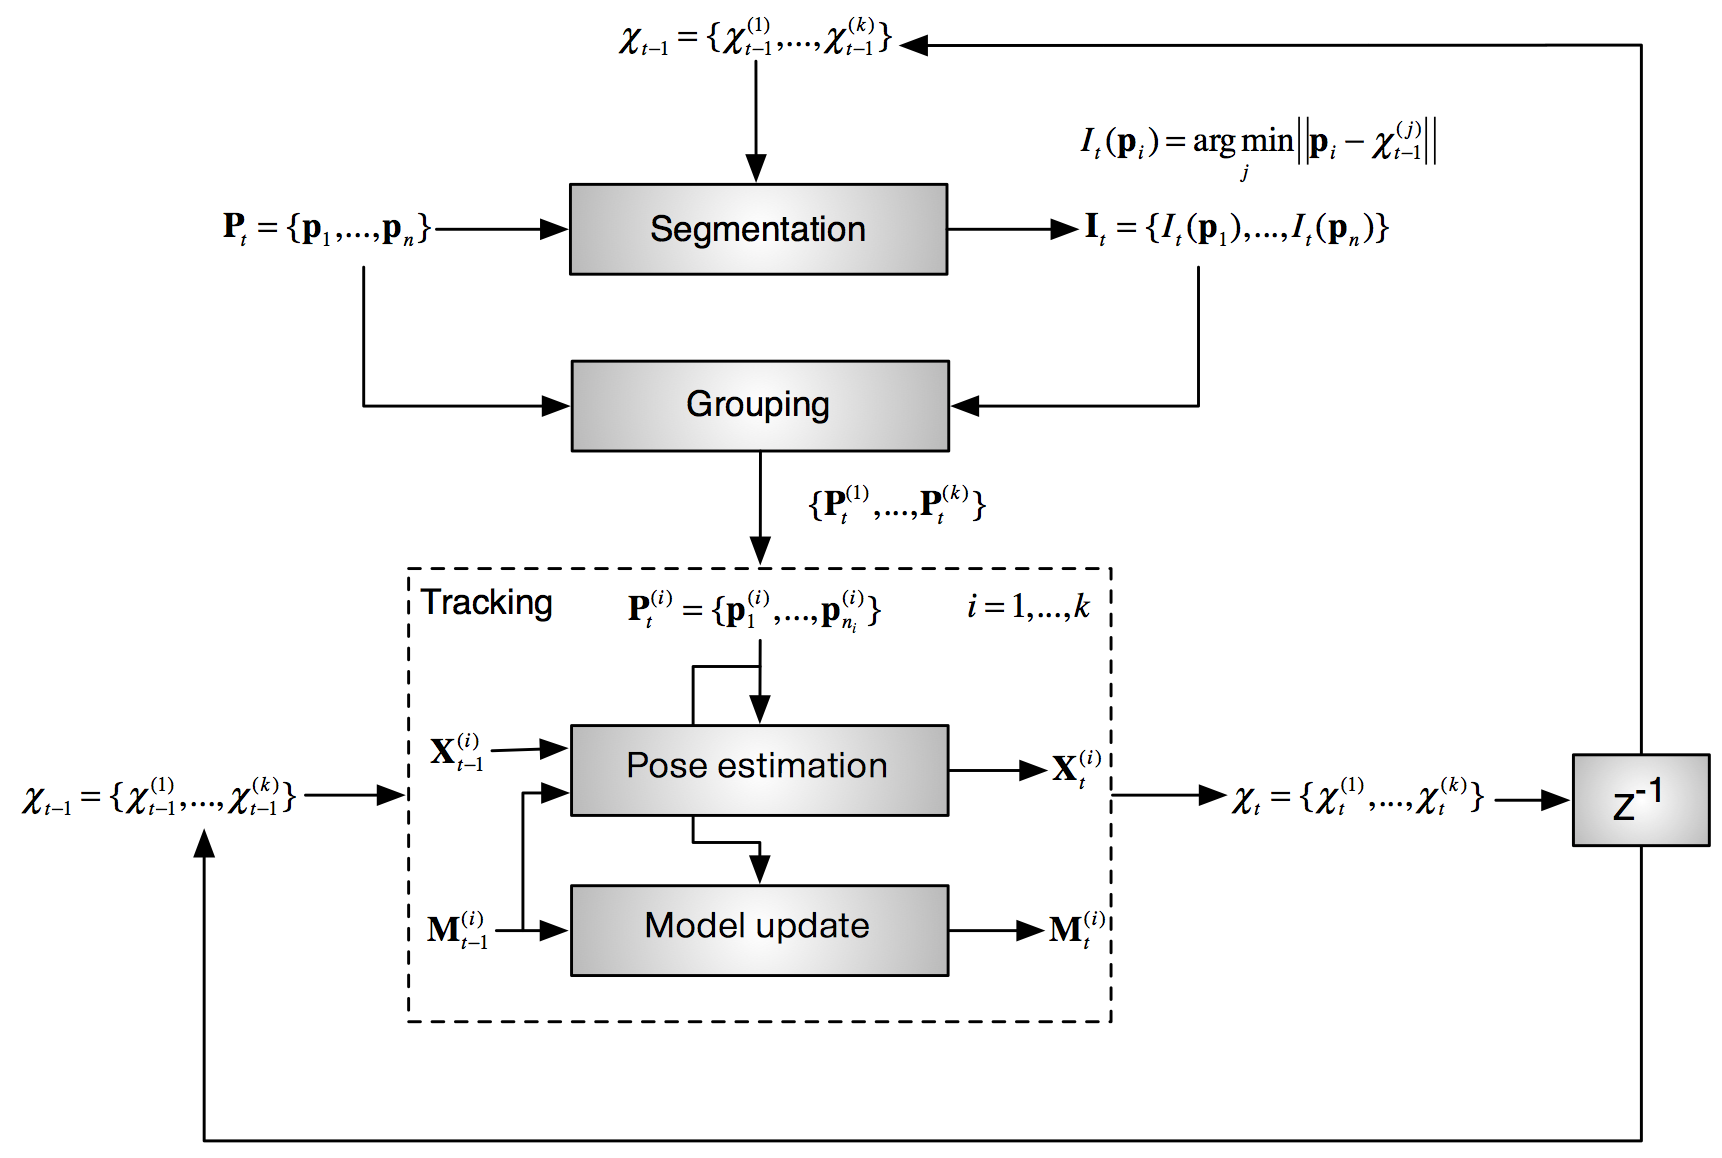
\includegraphics[width=\linewidth]{fig/smost_framework.png}
	\caption{A conceptual block diagram of SMOST}
	\label{fig:concept}
\end{figure}

%_____________________________________________________
\chapter{Installation}

This chapter explains how to install PMOT software and compile it on your computer. Because it needs some required 3rd party dependent libraries, please follow carefully step by step.

\section{System requirements}
 
In order to guarantee the performance reported in our papers, a system similar to or better than following specifications is required. 

\begin{itemize} 
	\item CPU: Intel Core i7-4790K CPU @ 4.00GHz $\times$ 8
	\item Memory: 16GByte
	\item GPU: GeForce GTX 660
	\item OS: Ubuntu 12.04 (precise) 64-bit	
	
\end{itemize} 

\section{Dependent libraries}
In order to successfully compile PMOT, the following 3rd party software or libraries are required.

\subsection{Robot Operating System (ROS)}
PMOT is running as a standalone node on ROS, at least ROS Hydro. It should be sure that ROS is successfully installed on your system and operating with no problem.
 
To install ROS Hydro, do the following in a Shell\footnote[6]{More details can be found in http://wiki.ros.org/hydro/Installation/Ubuntu}:

\begin{verbatim}
  wget https://raw.githubusercontent.com/ros/rosdistro/master/ros.key 
  sudo apt-key add ros.key
  sudo apt-get update
  sudo apt-get install ros-hydro-desktop-full
\end{verbatim}}

After successful installation, you should make the ROS setup file be called once you open a new shell.

Open \verb|.bashrc| file:
\begin{verbatim}
  cd ~/
  gedit .bashrc
\end{verbatim}

Add this line at the bottom line of the .bashrc file:
\begin{verbatim}
  source /opt/ros/hydro/setup.bash
\end{verbatim}

\subsection{CUDA}
PMOT requires GPU processing, which is implemented by using CUDA library. 
Go to the CUDA download page and install the recent version of CUDA (higher than ver 6.5)\footnote[7]{https://docs.nvidia.com/cuda/cuda-getting-started-guide-for-linux/\#ubuntu-installation}:  \hyperlink{https://developer.nvidia.com/cuda-downloads}{https://developer.nvidia.com/cuda-downloads}

\subsection{Point cloud library (PCL)}
One of the main dependent library of PMOT is the point cloud library (PCL)\footnote[8]{http://pointclouds.org/}. The current version of PMOT is using experimental version of PCL 1.8. Unfortunately the official release version is not available on the current time (13.03.2015), but you can download and compile it from source code as follows\footnote[9]{http://pointclouds.org/downloads/source.html}:
\begin{verbatim}
  git clone https://github.com/PointCloudLibrary/pcl pcl-trunk
  cd pcl-trunk && mkdir build && cd build
  cmake -DCMAKE_BUILD_TYPE=Release .. 
  make
  sudo make install
\end{verbatim}}

\subsection{Qt4}
Qt\footnote[9]{http://qt-project.org/} is one of the most widely used and well structured cross-platform library especially for Graphic User Interface (GUI) system. Although PMOT does not have GUI system inside, another necessary ROS node that we privide, \verb|camcalib|, should be built with Qt4. It will be explained in the next section.
  
Ubuntu 12.04 originally includes Qt4 as a default system library. If you have it then skip this step. 
\begin{verbatim}
  sudo apt-get install qt4-dev-tools
\end{verbatim}}


\subsection{VXL}
VXL is C++ libraries for computer vision research and implementation\footnote[10]{http://vxl.sourceforge.net/}, which includes libraries for numerics (vnl), imaging(vil), vgl(geometry), and so on. In PMOT, some code is written with vnl so that it could easily solve an optimization problem. 

First download vxl-1.17 sorce code here: http://vxl.sourceforge.net/\#download.
Unzip the source file in your any project folder (let's call it \verb|$VXLSRC|),
then follows the next steps to install it using cmake\footnote[11]{http://vxl.sourceforge.net/releases/install-release.html}. 

\begin{verbatim}
  cd $VXLSRC
  mkdir build
  cd build
  ccmake ..
  make 
  sudo make install
\end{verbatim}}

Note that, when you face to some errors to install whole packages in VXL, just carefully try to install vnl library successfully. 

 
\subsection{Lemon}
Lemon\footnote[12]{http://lemon.cs.elte.hu/trac/lemon} is one of the important libraries to implement graph-based algorithms in PMOT. Here is how to get and install it on your system. 

Download lemon-1.3.1 source code here: http://lemon.cs.elte.hu/trac/lemon/wiki/Downloads.

Installation steps\footnote[13]{http://lemon.cs.elte.hu/trac/lemon/wiki/InstallLinux} are almost similar to them of vxl above. Let's call you download and unzip source files in the project folder named \verb|$LEMONSRC|).
Then follow this. 

\begin{verbatim}
  cd $LEMONSRC
  mkdir build
  cd build
  ccmake ..
  make 
  sudo make install
\end{verbatim}}

\section{Compiling and building PMOT}
After installing all dependencies as introduced above, now you are ready to compile and build PMOT software. Additionally in order to get point-cloud data from an RGB-D camera, the second section will introduce our camera calibration program (camcalib) to convert sensor data from the camera coordinate to the world coordinate. 

When you get PMOT source code in our webpage\footnote[14]{http://www.hri.ei.tum.de/pmot}, unzip the files in your project folder, called \verb|$PMOTSRC| here. 
The subfolders in \verb|$PMOTSRC| are listed as follows.
\begin{itemize}
	\item \verb|/pmot|: PMOT source files.
	\item \verb|/camcalib|: Camera calibration (camcalib) source files.
	\item \verb|/doc|: Latex source files of this document and class description document generated by doxygen. 
\end{itemize}

Make sure that your project folder is included in the \verb|ROS_PACKAGE_PATH| which is defined in the ubuntu environment variables. If not, run the following code in the current shell. 
\begin{verbatim}
  export ROS_PACKAGE_PATH=$PMOTSRC:$ROS_PACKAGE_PATH
\end{verbatim}}

The above command is valid only in the current shell. If you like to apply the setting every time you open a new shell, open \verb|.bashrc| file as follows and add the command at the bottom line. 
\begin{verbatim}
  cd ~/
  gedit .bashrc
\end{verbatim}

Now you are ready to compile PMOT and camcalib. In order for PMOT source code to be compiled on cross platform policy (write on one system and compile on multiple systems.), it was written be using CMake\footnote[15]{http://www.cmake.org/}. You can use any CMake-available tools for compiling and building PMOT. Here, I recommend QtCreator and followings are how to install and compile PMOT with it. 

To install QtCreator on ubuntu, run the command on the shell. 
\begin{verbatim}
  sudo apt-get install qtcreator
\end{verbatim}
 
After installed, run QtCreator on a new shell that already includes ROS-related environment setup. 
\begin{verbatim}
  qtcreator
\end{verbatim}

\subsection{PMOT}
To open PMOT project, follow the steps in QtCreator. 
\begin{figure}[t]
	\centering
	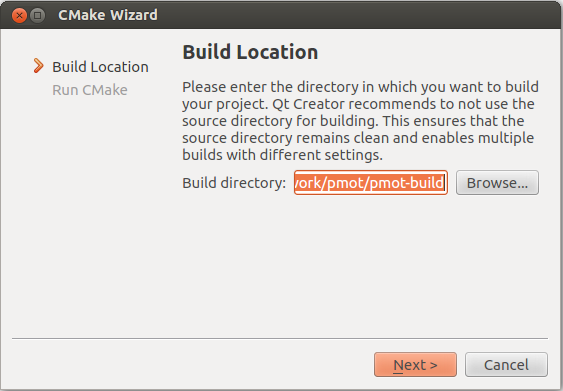
\includegraphics[width=0.5\linewidth]{fig/cmakewizard.png}
	\caption{CMake Wizard}
	\label{fig:cmakewizard}
\end{figure}

\begin{figure}[t]
	\centering
	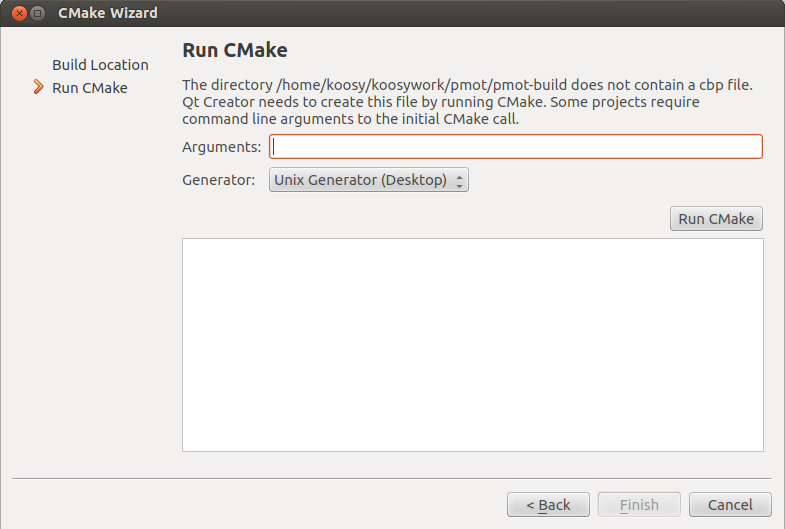
\includegraphics[width=0.5\linewidth]{fig/runcmake.png}
	\caption{Run CMake}
	\label{fig:runcmake}
\end{figure}
\begin{enumerate}
	\item Go to the top menu and press \verb|File| $\rightarrow$ \verb|Open File or Project|.
	\item Select \verb|CMakeLists.txt| in the folder \verb|$PMOTSRC/pmot|. Then, you will see a pop up window named CMake Wizard as Fig. \ref{fig:cmakewizard}.
	\item Select the \verb|build directory| where you want to make auxiliary files during the building process. These files are not necessary after building step so you can select any folder for this and delete it afterwards. 
	I used \verb|$PMOTSRC/pmot-build| for this example. 
	\item Click \verb|Next| button. Then, you will see the window to run cmake as shown in Fig. \ref{fig:runcmake}
	\item Click \verb|Run CMake| button.
	\item If your project is successfully built by CMake, you can see the \verb|Finish| button is turn to red. Then press the \verb|Finish| button. 
\end{enumerate}

\begin{figure}[t]
	\centering
	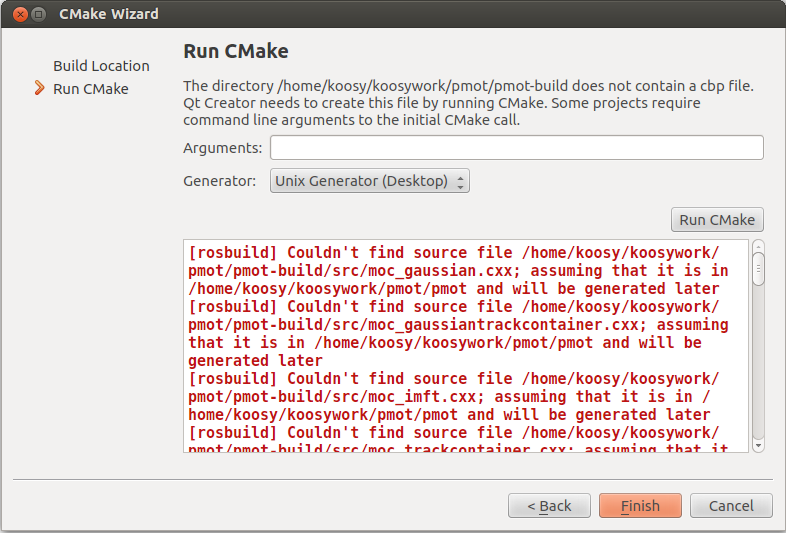
\includegraphics[width=0.5\linewidth]{fig/cmakefinish.png}
	\caption{Finish CMake}
	\label{fig:cmakefinish}
\end{figure}

After finishing CMake, PMOT project is loaded in your QtCreator. You can check which files are included in your project in the left panel as shown in Fig. \ref{fig:leftpanel}.
\begin{figure}[h]
	\centering
	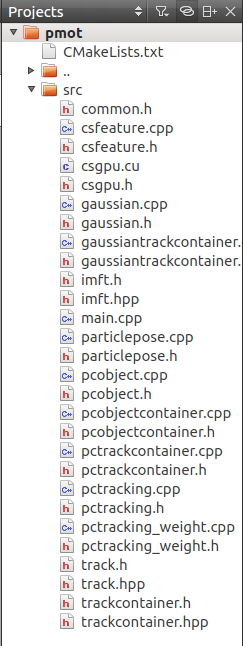
\includegraphics[width=0.2\linewidth]{fig/leftpanel.png}
	\caption{PMOT include files}
	\label{fig:leftpanel}
\end{figure}

Before compiling PMOT, let's check the content in CMakeLists.txt which describes all necessary settings for PMOT.
Click CMakeLists.txt file on the left panel, then you can see the file in the main panel as follows.

\begin{boxedverbatim}
cmake_minimum_required(VERSION 2.4.6)
include($ENV{ROS_ROOT}/core/rosbuild/rosbuild.cmake)
rosbuild_init()

set(EXECUTABLE_OUTPUT_PATH ${PROJECT_SOURCE_DIR}/bin)
set(LIBRARY_OUTPUT_PATH ${PROJECT_SOURCE_DIR}/lib)

## Include files
set( sources
src/main.cpp
src/pctracking.cpp
src/pctracking_weight.cpp
src/particlepose.cpp
src/csfeature.cpp

src/pcobject.cpp
src/pcobjectcontainer.cpp
src/track.hpp
src/trackcontainer.hpp
src/pctrackcontainer.cpp

src/imft.hpp
src/gaussian.cpp
src/gaussiantrackcontainer.cpp
)

set( headers
src/pctracking.h
src/pctracking_weight.h
src/particlepose.h
src/csfeature.h
src/csgpu.h

src/pcobject.h
src/pcobjectcontainer.h
src/track.h
src/trackcontainer.h
src/pctrackcontainer.h
src/imft.h
src/gaussian.h
src/gaussiantrackcontainer.h
)
\end{boxedverbatim}

\begin{boxedverbatim}
## CUDA
FIND_PACKAGE(CUDA REQUIRED)
INCLUDE(FindCUDA)
CUDA_ADD_LIBRARY (csgpulib src/csgpu.cu src/csgpu.h)
CUDA_ADD_EXECUTABLE(pmot src/csgpu.cu)

## VXL
include_directories(
/usr/local/include/vxl/vcl
/usr/local/include/vxl/core
/usr/local/include/vxl/core/vnl/algo
/usr/local/include/vxl/v3p/netlib
)
FIND_PACKAGE(VXL)

## PCL 1.8
find_package(PCL 1.8 REQUIRED)
include_directories(BEFORE ${PCL_INCLUDE_DIRS})
link_directories(${PCL_LIBRARY_DIRS})
add_definitions(${PCL_DEFINITIONS})
if (NOT PCL_FOUND)
MESSAGE(FATAL_ERROR "PCL not found.\n")
endif (NOT PCL_FOUND)

## Qt
find_package(Qt4)
set(QT_USE_QTOPENGL TRUE)
include(${QT_USE_FILE})

## ROS build
rosbuild_add_executable(pmot ${sources} ${headers})
target_link_libraries(pmot vnl_algo vnl vcl QtGui ${PCL_LIBRARIES})
SET_TARGET_PROPERTIES(pmot PROPERTIES LINK_FLAGS -L${PCL_LIBRARY_DIRS})
\end{boxedverbatim}
\\

Let's look at CMakeLists.txt inside by breaking down to the following separated parts. 

The first part is a general step to use \verb|rosbuild| tool in the project. 
\begin{verbatim}
  cmake_minimum_required(VERSION 2.4.6)
  include($ENV{ROS_ROOT}/core/rosbuild/rosbuild.cmake)
  rosbuild_init()
  
  set(EXECUTABLE_OUTPUT_PATH ${PROJECT_SOURCE_DIR}/bin)
  set(LIBRARY_OUTPUT_PATH ${PROJECT_SOURCE_DIR}/lib)
\end{verbatim}

Next part defines C++ source and header files that are included in the project. For professional users, if you want to add another files in the project, please add the file names here.    
\begin{verbatim}
  ## Includes
  set( sources
  src/main.cpp
  src/pctracking.cpp
  src/pctracking_weight.cpp
  src/particlepose.cpp
  src/csfeature.cpp

  src/pcobject.cpp
  src/pcobjectcontainer.cpp
  src/track.hpp
  src/trackcontainer.hpp
  src/pctrackcontainer.cpp

  src/imft.hpp
  src/gaussian.cpp
  src/gaussiantrackcontainer.cpp
  )

  set( headers
  src/pctracking.h
  src/pctracking_weight.h
  src/particlepose.h
  src/csfeature.h
  src/csgpu.h

  src/pcobject.h
  src/pcobjectcontainer.h
  src/track.h
  src/trackcontainer.h
  src/pctrackcontainer.h
  src/imft.h
  src/gaussian.h
  src/gaussiantrackcontainer.h
  )
\end{verbatim}

This looks for the installed CUDA libraries and includes required header files.
\begin{verbatim}
  FIND_PACKAGE(CUDA REQUIRED)
  INCLUDE(FindCUDA)
\end{verbatim}

These two lines are important to build GPU-related source codes in PMOT, which are \verb|csgpu.cu| and \verb|csgpu.h|. As a result of this setting, a new library file (\verb|libcsgpulib.so|) will be generated in \verb|$PMOTSRC\pmot\lib|.
\begin{verbatim}
  CUDA_ADD_LIBRARY (csgpulib src/csgpu.cu src/csgpu.h)
  CUDA_ADD_EXECUTABLE(pmot src/csgpu.cu)
\end{verbatim}

Next three parts are for including other dependencies, VXL, PCL, and Qt, which are already installed in your system as introduced in the section 2.2.
\begin{verbatim}
  ## VXL
  include_directories(
  /usr/local/include/vxl/vcl
  /usr/local/include/vxl/core
  /usr/local/include/vxl/core/vnl/algo
  /usr/local/include/vxl/v3p/netlib
  )
  FIND_PACKAGE(VXL)

  ## PCL 1.8
  find_package(PCL 1.8 REQUIRED)
  include_directories(BEFORE ${PCL_INCLUDE_DIRS})
  link_directories(${PCL_LIBRARY_DIRS})
  add_definitions(${PCL_DEFINITIONS})
  if (NOT PCL_FOUND)
  MESSAGE(FATAL_ERROR "PCL not found.\n")
  endif (NOT PCL_FOUND)

  ## Qt
  find_package(Qt4)
  set(QT_USE_QTOPENGL TRUE)
  include(${QT_USE_FILE})
\end{verbatim}

The final part is to link all files and libraries to build ros node with the \verb|rosbuild| tool. 
\begin{verbatim}
  ## ROS build
  rosbuild_add_executable(pmot ${sources} ${headers})
  target_link_libraries(pmot vnl_algo vnl vcl QtGui ${PCL_LIBRARIES})
  SET_TARGET_PROPERTIES(pmot PROPERTIES LINK_FLAGS -L${PCL_LIBRARY_DIRS})
\end{verbatim}

To compile and build PMOT, press \verb|crtl+b| in QtCreator. If it is successfully built it will show no errors, and the binary file, \verb|pmot| will be found in \verb|$PMOTSRC/pmot/bin|. 
\subsection{Camera calibration (camcalib)}
To open camcalib project in QtCreator, follow the steps similar those of PMOT. 

\begin{enumerate}
	\item Go to the top menu and press \verb|File| $\rightarrow$ \verb|Open File or Project|.
	\item Select \verb|CMakeLists.txt| in the folder \verb|$PMOTSRC/camcalib|.  
	\item Select the \verb|build directory| where you want to make auxiliary files during the building process. 
	I used \verb|$PMOTSRC/camclib-build| for this example. 
	\item Click \verb|Next| button. 
	\item Click \verb|Run CMake| button. If your project is successfully built by CMake, you can see the \verb|Finish| button is turn to red. 
	\item Press the \verb|Finish| button. 
\end{enumerate}

Similar to the above PMOT, let's look at CMakeLists.txt of camcalib for better understanding of the source code structure.
Here I will explain the only different part from the CMakeLists.txt file of PMOT.

The \verb|##include| part shows C++ source and header files in camcalib. Note that this also needs to include \verb|${CMAKE_CURRENT_BINARY_DIR}| to load the generated \verb|ui_*| files in the build directory, which means that \verb|$PMOTSRC/camclib-build| should not be deleted after building project.
\begin{verbatim}
  ## include
  set( sources
  src/calibrationOneCam.cpp
  src/mainwindow.cpp
  src/dialogcalibration.cpp
  src/ckinectcalibration.cpp
  src/ckinectthread.cpp
  src/ckinecttfpublisher.cpp
  )  

  set( headers
  src/mainwindow.h
  src/dialogcalibration.h
  src/ckinectcalibration.h
  src/ckinectthread.h
  src/ckinecttfpublisher.h
  )

  include_directories(
  ${CMAKE_CURRENT_BINARY_DIR}
  )
\end{verbatim}

Same as PMOT, compile and build camcalib project by pressing \verb|crtl+b|. The binary file \verb|camcalib| will be generated in \verb|$PMOTSRC/camcalib/bin|.
%_____________________________________________________
\chapter{Program Execution}

After PMOT and camcalib are successfully compiled and built, now it is ready to execute those programs to get the results. This chapter will explain the execution steps first camcalib and second PMOT, because camcalib deals with pre-process of the sensor data to provide input data for PMOT. 

\section{Camera calibration (camcalib)}

Our camera calibration probram (camcalib) changes sensor data nothing but to different coordinate system. 
Fig. \ref{fig:camcalib} shows the transformed input point-cloud that is measured from \verb|camera_link| frame to \verb|origin| on the table.
At each time step, camcalib transforms the input point-cloud data according to the predefined relative pose of the camera from the origin. 
Because it is not easy to find the relative pose values by users, camcalib provides GUI tool to adjust the pose values interactively and dynamically with ROS 3D visualization tool (RVIZ). 
In addition to the manual calibration, camcalib provides auto calibration with an arbitrary black-white checker board, specification of which can be defined.
\begin{figure}[b]
	\centering
	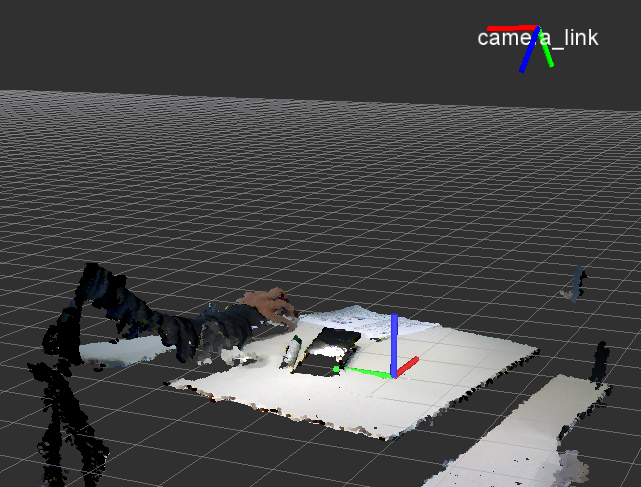
\includegraphics[width=0.45\linewidth]{fig/camcalib.png}
	\caption{Camera calibration coordinates}
	\label{fig:camcalib}
\end{figure}

\subsection{Setting parameters}
One of the benefit of using ROS is that it allows a parameter server to save and load several parameter variables outside of ROS nodes and dynamically share them for all nodes.
Here, we use the server to define the relative pose so that transformation messages (TF) can be dynamically generated as a user changes its parameters in GUI.

There are two parameter files in \verb|$PMOTSRC/camcalib|: \verb|param_camera.yaml| and \verb|param_checkboard.yaml|.
As the names indicate, the first one defines the current camera pose from origin, and the second stores the size of checker board that will be used for auto calibration. The details of the use of those values will be explained in the next section.

Let's look at the first parameter \verb|param_camera.yaml|.
\begin{verbatim}
  /dhri/calibrationOneCam/camera/x: 0.593
  /dhri/calibrationOneCam/camera/y: -0.041
  /dhri/calibrationOneCam/camera/z: 0.584
  /dhri/calibrationOneCam/camera/yaw: 82.15
  /dhri/calibrationOneCam/camera/pitch: 1.12
  /dhri/calibrationOneCam/camera/roll: -136.68
\end{verbatim}

The numbers are examples, but you can see that there are six float-typed parameters to define the camera pose: x,y,z,yaw,pitch, and roll. 
The file can be changed not only by manual editing but also by the camcalib program. You can check how the values are changed after running camcalib.

The second file \verb|param_checkboard.yaml| includes following parameters.
\begin{verbatim}
  /dhri/calibrationOneCam/checkboard/nW: 8
  /dhri/calibrationOneCam/checkboard/nH: 6
  /dhri/calibrationOneCam/checkboard/size: 0.1083
\end{verbatim}

\verb|nW| means number of checkers in the width direction while \verb|nH| indicates number of checkers in the height direction. \verb|size| defines the size of each side of the checker in $m$.
Fig. \ref{fig:checker} shows an example of usable $5 \times 5$ checker pattern.
\begin{figure}[b]
	\centering
	
\includegraphics[width=0.25\linewidth]{fig/checker.png}
	\caption{An example of usable checker pattern}
	\label{fig:checker}
\end{figure}

\subsection{Execution}

Before running camcalib, check that \verb|openni2| is already installed in your ROS. If not, run these two lines to install it. 

\begin{verbatim}
  sudo apt-get install ros-hydro-openni2-camera
  sudo apt-get install ros-hydro-openni2-launch
\end{verbatim}

camcalib needs to run a set of openni2 existing nodes and several commands to set parameters that are introduced above.
Another useful ros tool, \verb|roslaunch|, enables to run a set of ros packages and parameters only with a single command.

Here, to run camcalib, you only need to run the following single command at any location on your shell. 
\begin{verbatim}
  roslaunch camcalib.launch
\end{verbatim}

Following list shows what the launch file automatically executes before runnning camcalib (only important parts are listed).
\begin{itemize}
	\item rgbd\_launch/manager.launch
	\item openni2\_laundh/device.launch
	\item rgbd\_launch/processing.launch
	\item rgbd\_launch/kinect\_frames.launch
	\item param\_camera.yaml
	\item param\_checkboard.yaml
\end{itemize}

When you launch camcalib, you will see a GUI window as shown in Fig. \ref{fig:camcalib_gui1}.

\begin{figure}[b]
	\centering
	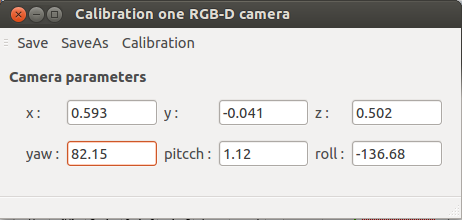
\includegraphics[width=0.5\linewidth]{fig/camcalib_gui1.png}
	\caption{The first GUI of camcalib}
	\label{fig:camcalib_gui1}
\end{figure}

Each value in \verb|camera parameters| is loaded from \verb|param_camera.yaml| file that are already loaded in the ros parameter server.

To show the camera and origin coordinates with the sensor point-cloud data, open a new RVIZ in a new shell. 

\begin{verbatim}
  rosrun rviz rviz
\end{verbatim}

To automatically configure RVIZ environment for camcalb, open a \verb|camcalib.rviz| file in \verb|$PMOTSRC/camcalib| (\verb|File| $\rightarrow$ \verb|Open Config|.).

\begin{figure}[t]
	\centering
	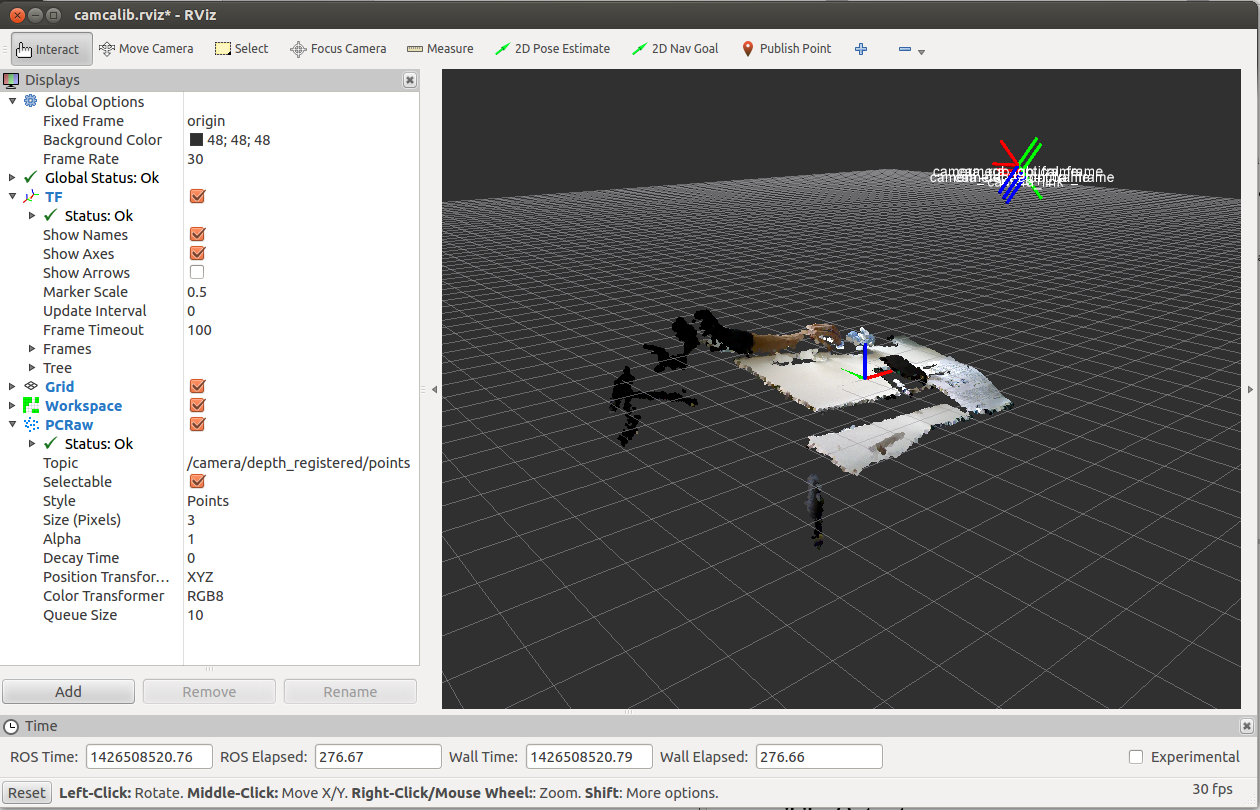
\includegraphics[width=\linewidth]{fig/camcalib_gui2.png}
	\caption{Transformed point-cloud and coordinates displayed in RVIZ}
	\label{fig:camcalib_gui2}
\end{figure}

As shown in Fig. \ref{fig:camcalib_gui2}, you can see the transformed point-cloud is displayed in RVIZ with its two coordinate systems (camera\_* and origin). Note that the first global option \verb|Fixed Frame| is assigned with \verb|origin|. 

Another important setting you have to notice is the name of point-cloud topic, \verb|/camera/depth_registered/points|, which is the same as the name of raw point-cloud data before transformation. This fact says that camcalib does not produce another new point-cloud data after transformation. Rather than that, it only produces transformation (TF) message between \verb|origin| and \verb|camera| so that subscribers can use the data as additional information to the original point-cloud. In RVIZ, it is clearly shown that you can see original measured point-cloud by changing the fixed frame name to one of the camera frames.  

There are two ways to calibrate camera poses: auto calibration with a checker board, and manual calibration with RVIZ. When you click \verb|Calibration| button in the window of Fig. \ref{fig:camcalib_gui1}, you can see another pop-up window that has two taps: Auto and Manual.
Unfortunately, the Auto calibration is not working in the current version. It will be updated soon. 

\begin{figure}[t]
	\centering
	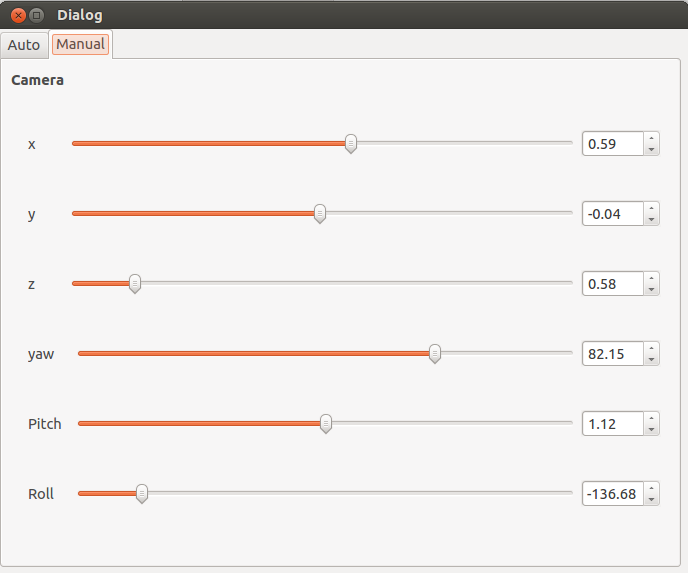
\includegraphics[width=0.5\linewidth]{fig/camcalib_gui3.png}
	\caption{Transformed point-cloud and coordinates displayed in RVIZ}
	\label{fig:camcalib_gui3}
\end{figure}

When you click 'Manual' tap, you will see six horizontal sliding bars as shown in Fig. \ref{fig:camcalib_gui3}.
By manipulating the bars, you can change the camera pose relative to the origin. Fig. \ref{fig:camcalib_manip} shows the two cases of changing x values. You can see the input poin-cloud is moving according to the camera poses. In this interactive way, you can adjust the camera pose exactly and delicately. 

After calibrating the camera pose, do not forget to save the pose values in the \verb|param_camera.yaml| file. This task can be done by pressing \verb|save| button on the main window in Fig. \ref{fig:camcalib_gui1}. You can also save the parameters with different names to different locations by using \verb|save as|. It is useful when you need to extract several different camera poses. 

\begin{figure}[b]
	\centering
	\subfloat[x = 0]{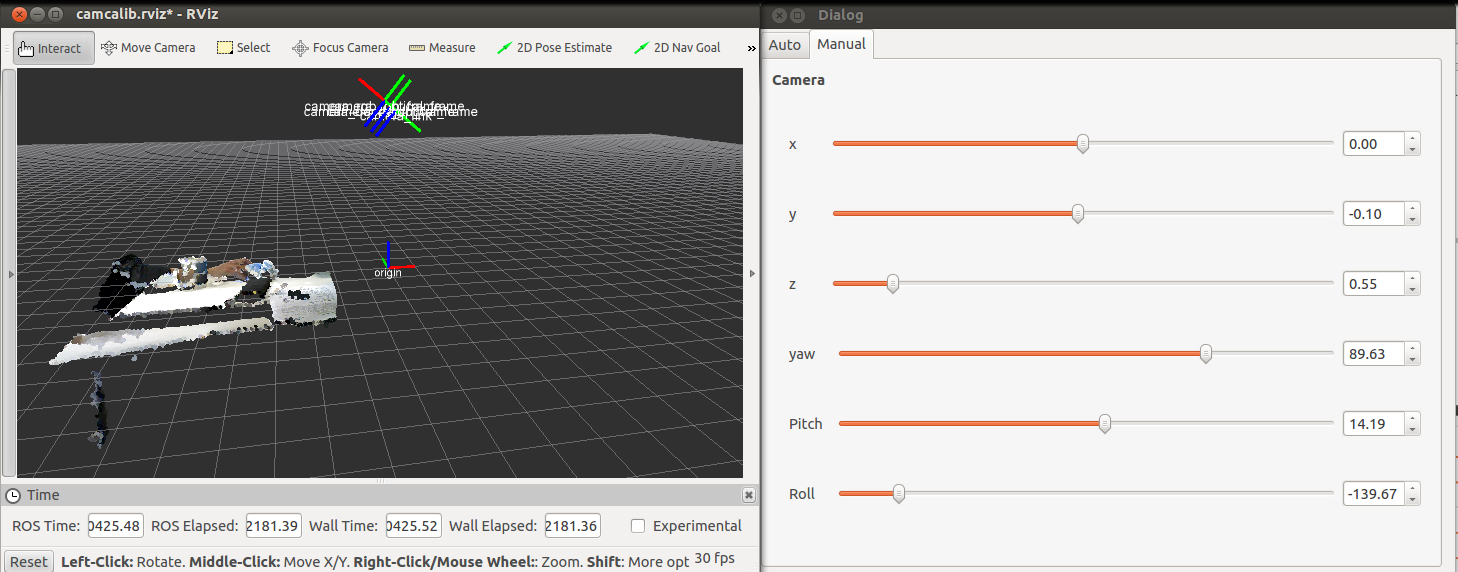
\includegraphics[width=0.45\linewidth]{fig/camcalib_gui4.png}%
		\label{fig_first_case}}
	\hfil
	\subfloat[x = 1.13]{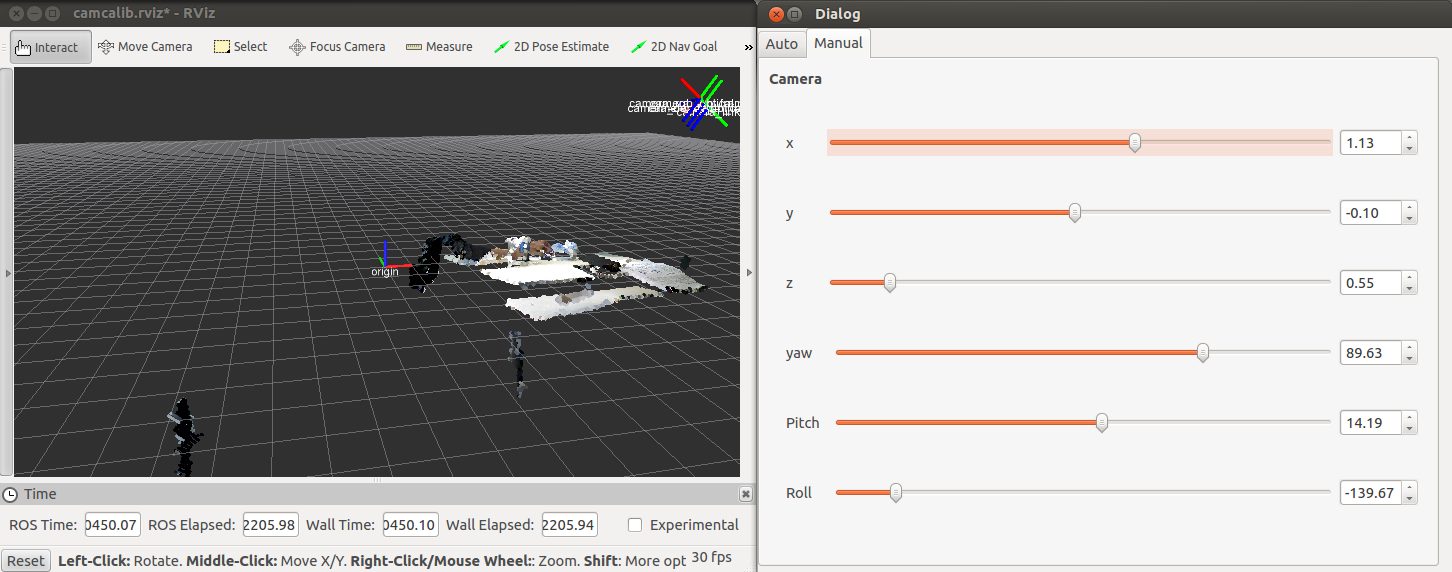
\includegraphics[width=0.45\linewidth]{fig/camcalib_gui5.png}%
		\label{fig_second_case}}
	\caption{Existing point-cloud object tracking softwares}
	\label{fig:camcalib_manip}
\end{figure}

\section{PMOT}

With camcalib program as a running ros node, PMOT can process the input point-cloud and produce several outputs. This chapter explains how to get PMOT be ready by setting required parameters, and how to subscribe its outputs. 

\subsection{Setting parameters}

As similar to camcalib above, PMOT also has several parameters to be set into the ros parameter server.  
Open the file \verb|param.yaml| in \verb|$PMOTSRC/pmot|.
\begin{verbatim}
  /dhri/multipleObjectTracking/sub/topic: '/camera/depth_registered/points'
  /dhri/multipleObjectTracking/frame/id: '/origin'
  /dhri/multipleObjectTracking/pub/points/trackID: '/dhri/points/trackID'
  /dhri/multipleObjectTracking/pub/points/filtered: '/dhri/points/filtered'
  /dhri/multipleObjectTracking/pub/points/segmented: '/dhri/points/segmented'
  /dhri/multipleObjectTracking/pub/markers/trackID: '/dhri/markers/trackID'
  /dhri/multipleObjectTracking/pub/markers/gaussians: '/dhri/markers/gaussians'
  /dhri/multipleObjectTracking/workspace/topic: '/dhri/workspace'
  /dhri/multipleObjectTracking/workspace/x: 0.
  /dhri/multipleObjectTracking/workspace/y: 0.
  /dhri/multipleObjectTracking/workspace/z: 0.
  /dhri/multipleObjectTracking/workspace/width: 0.5
  /dhri/multipleObjectTracking/workspace/height: 0.5
  /dhri/multipleObjectTracking/workspace/zheight: 1.
  /dhri/multipleObjectTracking/param/samplingRatio: 5
  /dhri/multipleObjectTracking/param/segmentTolerance: 0.05
  /dhri/multipleObjectTracking/param/buffernum: 1
  /dhri/multipleObjectTracking/gpu/usegpu:  true
  /dhri/multipleObjectTracking/gpu/particlenumber: 500
  /dhri/multipleObjectTracking/gpu/gridsize: 0.02
  /dhri/multipleObjectTracking/gpu/newratio: 10.0
\end{verbatim}

The first parameter is the topic name of the input point-cloud. As you saw in \ref{fig:camcalib_gui2}, the name \verb|/camera/depth_registered/points| is same as the point-cloud topic from the openni2 launch file. The second parameter is the origin frame name that is defined in camcalib program. 
From the 3rd to 7th parameters define output ros topics that are published by PMOT. Each data will be explained in the next section. 
From the 8th to 14th parameters are involved in the 3D working space where the input point-cloud is filtered out. From 15th to final parameters are main setting values for PMOT, which are listed below. 

\begin{itemize}
	\item{\verb|samplingRatio|}: This is downsampling distance in $mm$ with which voxelgrid filter in pcl \cite{Rusu_ICRA2011_PCL} is performed to the input point-cloud in the working space. 
	\item{\verb||segmentTolerance|}: In order to segment the filtered point-cloud to individual objects, euclidean distance-based segmentation in \cite{Rusu_ICRA2011_PCL} is performed initially. The parameter is a minimum distance between point-cloud segments that are separated. 
	\item{\verb|buffernum|}: This is the buffer size to subscribe input point-cloud. If it sets to 1, it means PMOT is operating unsynchronously, which only cares recently arrived data. If you want to use PMOT as a real-time process without any delay, set this to 1. If you want to use PMOT in off-line but synchronous process, set this to enough value as much as your memory is available, e.g. 1000.  
	\item{\verb|usegpu|}: This bool-type variable (true/false) indicates whether GPU is available or not in your system. Note that, without GPU, real-time tracking (21fps) reported in \cite{li2015realtime} is not available. 
	\item{\verb|particlenumber|}: This is the number of particles in the particle filter for the pose estimation. Experimentally-obtained optimal number is 100 as reported in \cite{li2015realtime}. 
	\item{\verb|gridsize|}: In \cite{li2015realtime}, we defined Joing Color-Spatial Descriptor to represent an arbitrary object from a point-cloud. As shown in Fig. \ref{fig:grid}, the point-cloud is divided as a set of 3D grids, the \verb|gridsize| defines the size of grid size $r$ in $m$. The size depends on the target object size, but $2cm$ is the optimal value in our experiments. 
	\item{\verb|newratio|}: As explained in Fig. \ref{fig:concept}, the internal object model, ${\bf{M}}_t^{(i)}$, is updated from the previous object model, ${\bf{M}}_{t-1}^{(i)}$, and the newly measured point-cloud, ${\bf{P}}_{t-1}^{(i)}$, at every time step. The ratio is the sampling proportion in $\%$ of the new point-cloud ${\bf{P}}_{t-1}^{(i)}$. Accordingly, $100-\verb|newratio|$ is the sampling proportion of ${\bf{M}}_{t-1}^{(i)}$ accordingly. The value is sensitive to the dynamics of the target objects. If the target changes its shape fast, the value should be large. However, the bigger value allows the more errors, which possibly causes robustness problem. In our experiments, under the value of $10$ is reasonable in general table-top object manipulation scenarios. 
\end{itemize}

\begin{figure}[b]
	\centering
	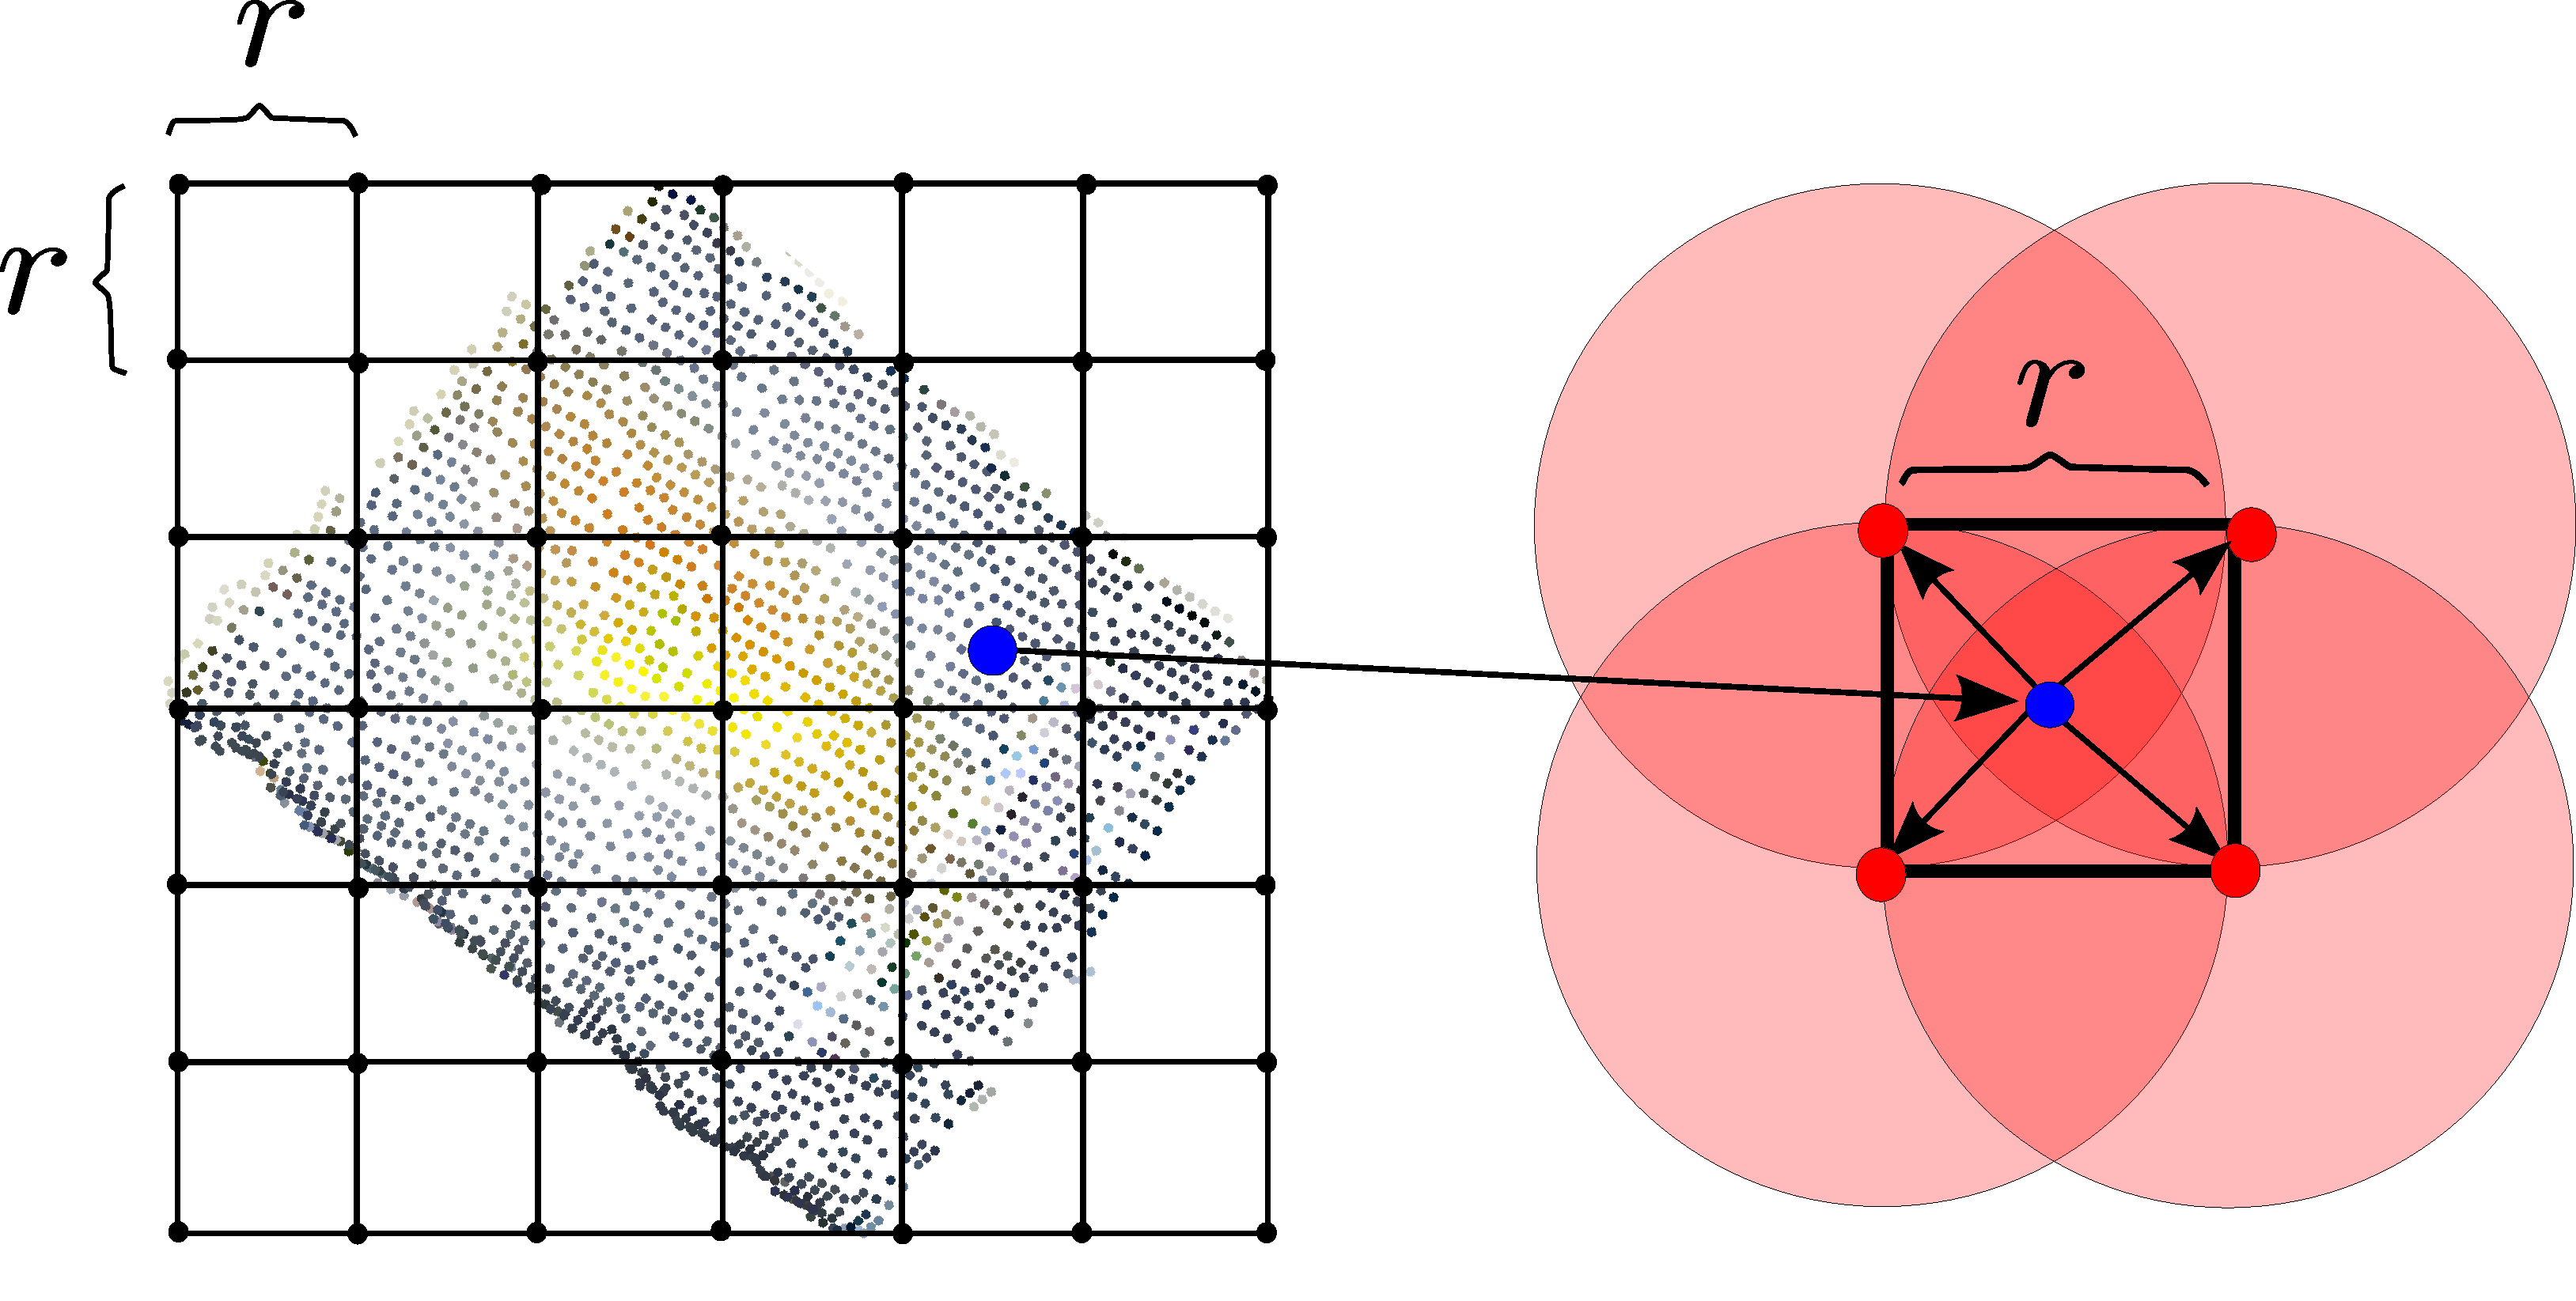
\includegraphics[width=0.7\linewidth]{fig/2dgrid.pdf}
	\caption{A set of grids to represent spatial distribution of an object.}
	\label{fig:grid}
\end{figure}

\subsection{Execution}
Before executing PMOT, the parameters above should be loaded first. With the roslaunch tool, the two steps can be easily launched by executing only one command below at any location on your shell. 
\begin{verbatim}
  roslaunch pmot pmot.launch
\end{verbatim}

The launch file \verb|pmot.launch| contains following scripts.
\begin{verbatim}
  <launch>
    <arg name="param" default="param.yaml" />
    <rosparam command="load" file="$(find pmot)/$(arg param)" />
    <node name="pmot" pkg="pmot" type="pmot" />
  </launch>
\end{verbatim}

After launching PMOT and there is no error message on your shell, now the outputs of PMOT are ready to be subscribed.
RVIZ is also an useful tool to test the PMOT outputs by subscribing them and visualizing the data in 3D space. Furthermore, multiple topics can be subscribed and visualized at the same time, or the other way around: multiple RVIZs can be executed at the same time, each of which subscribes one topic. Either way is good to examine and compare multiple outputs.

To run RVIZ, first follow the command:
\begin{verbatim}
  rosrun rviz rviz
\end{verbatim}

To automatically configure RVIZ environment for PMOT, open a \verb|pmot.rviz| file in \verb|$PMOTSRC/pmot| (\verb|File| $\rightarrow$ \verb|Open Config|.).

\subsubsection{Filtered point-cloud}

\begin{figure}[b]
	\centering
	\subfloat[Input point-cloud data]{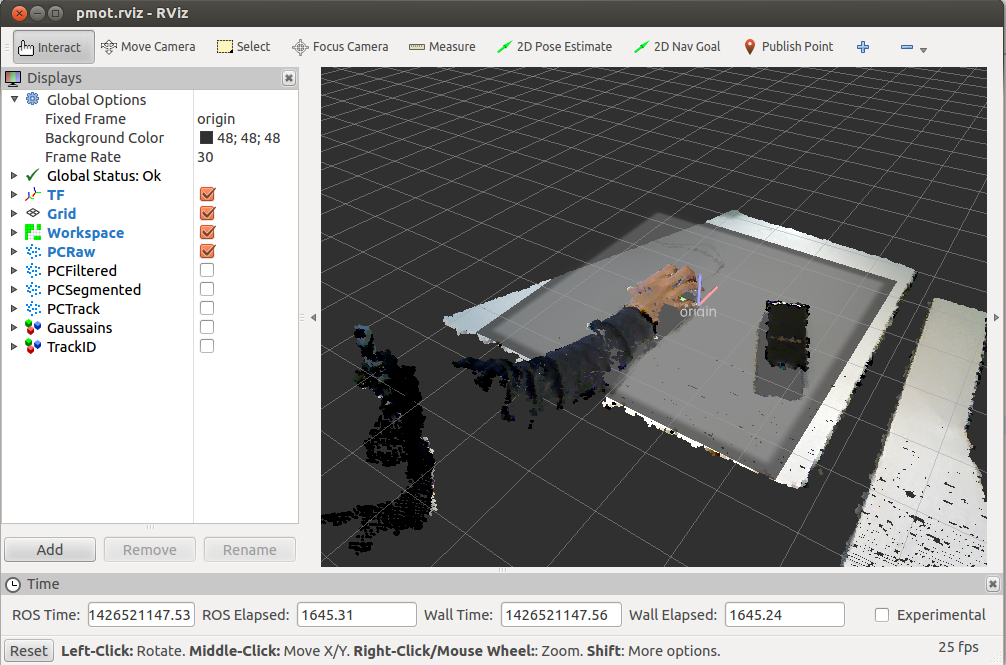
\includegraphics[width=0.45\linewidth]{fig/pmot_raw.png}%
		\label{fig:pmot_raw}}
	\hfil
	\subfloat[Filtered point-cloud in the work space]{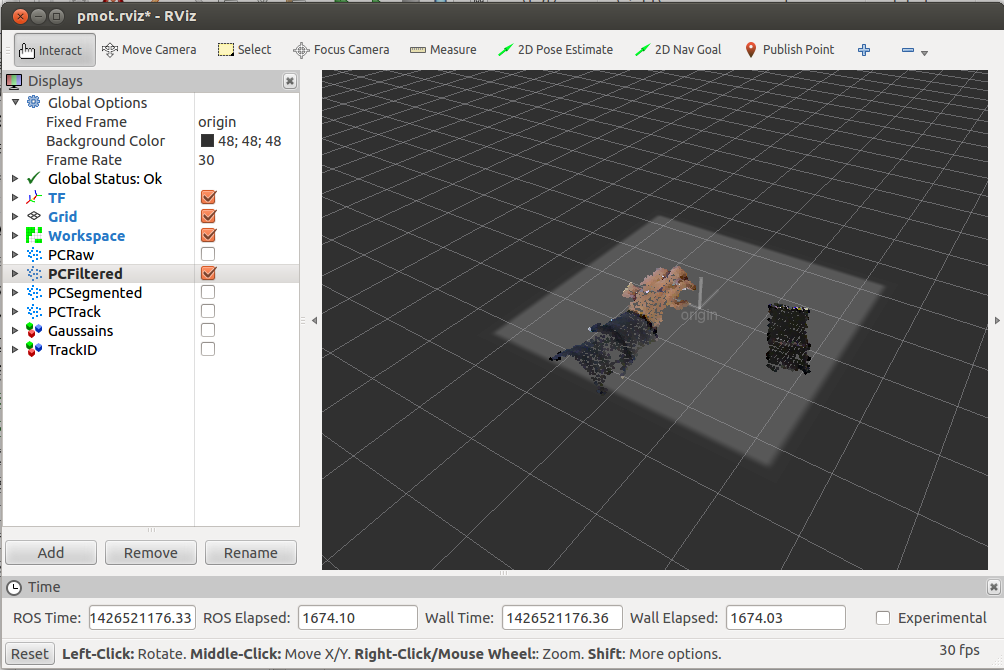
\includegraphics[width=0.45\linewidth]{fig/pmot_filtered.png}%
		\label{fig:pmot_filtered_workspace}}
	\caption{Existing point-cloud object tracking softwares}
	\label{fig:pmot_filtered}
\end{figure}
Let's check the first output, filtered point-cloud. The filtering is done by two steps: cutting out unnecessary part (outside of the working space) in the input point-cloud, and downsampling using the voxelgrid filter.

Fig. \ref{fig:pmot_filtered} shows the result of the filtered point-cloud comparing to the input point-cloud. You can see the point-cloud outside of the working space is cut out and the filtered one is less dense than the original one. 
The topic name of the filtered point-cloud is defined in the parameter file as follows: 
\begin{verbatim}
  /dhri/multipleObjectTracking/pub/points/filtered: '/dhri/points/filtered'
\end{verbatim}

The working space is defined as a 3D box, which is specified in the parameter file. 
\begin{verbatim}
  /dhri/multipleObjectTracking/workspace/topic: '/dhri/workspace'
  /dhri/multipleObjectTracking/workspace/x: 0.
  /dhri/multipleObjectTracking/workspace/y: 0.
  /dhri/multipleObjectTracking/workspace/z: 0.
  /dhri/multipleObjectTracking/workspace/width: 0.5
  /dhri/multipleObjectTracking/workspace/height: 0.5
  /dhri/multipleObjectTracking/workspace/zheight: 1.
\end{verbatim}
Here in RVIZ, only 2D surface is displayed but you can imagine the actual working space is $1m$ height.

\subsubsection{Segmented point-cloud}

The second output is the initial segmented point-cloud. This is the result of euclidean clustering to segment each object individual only by location information. 
Even though this information is not final result of PMOT and looks noisy, it is good reference to show how model-free object segmentation is difficult to solve. Thus, it is useful to show the final results with the initial segmentation results.
Fig. \ref{fig:pmot_segmented} shows the initial segmentation results in the two cases. When the two objects are separated as shown in Fig. \ref{fig:pmot_segmented_separated}, the initial segmentation results in clear separations. However, as shown in Fig. \ref{fig:pmot_segmented_merged}, when the two objects are contacted, the euclidean clustering cannot separate the two individual objects.
\begin{figure}[b]
	\centering
	\subfloat[The separation case ]{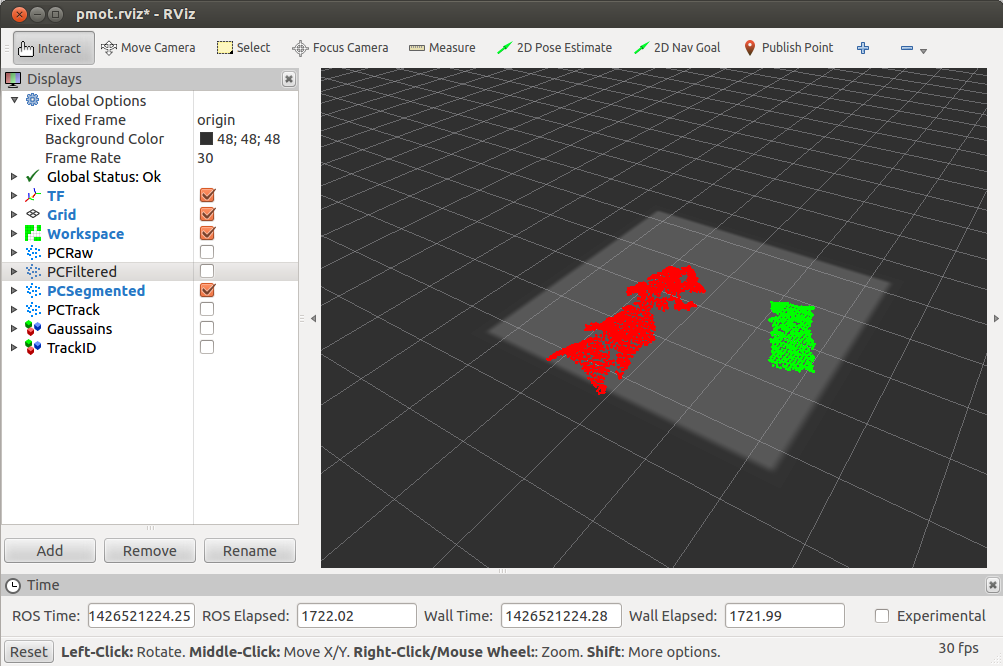
\includegraphics[width=0.45\linewidth]{fig/pmot_segmented_separated.png}%
		\label{fig:pmot_segmented_separated}}
	\hfil
	\subfloat[The contact case]{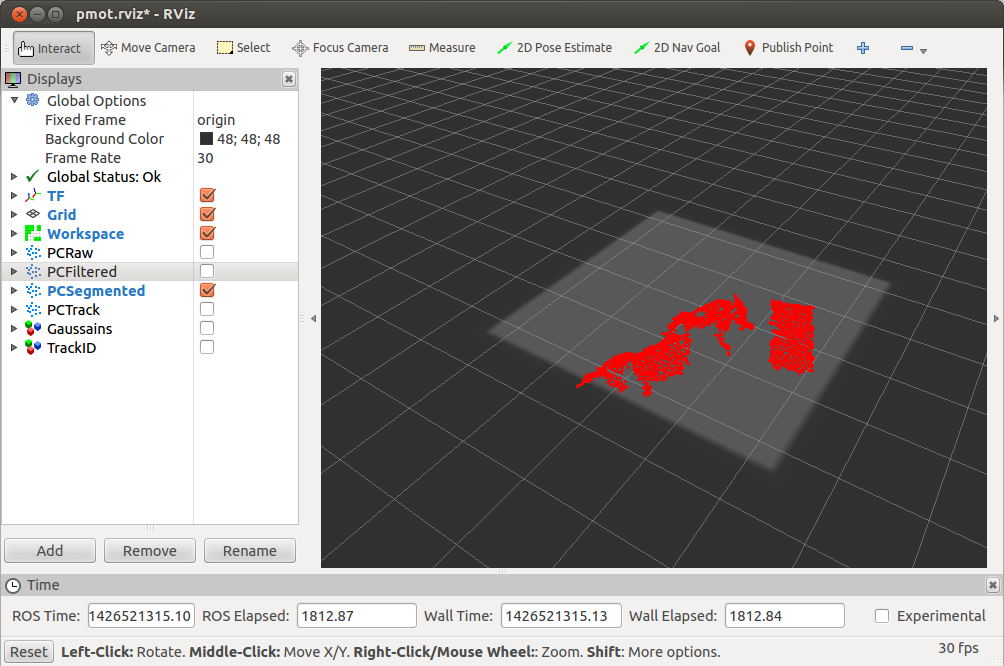
\includegraphics[width=0.45\linewidth]{fig/pmot_segmented_merged.png}%
		\label{fig:pmot_segmented_merged}}
	\caption{Existing point-cloud object tracking softwares}
	\label{fig:pmot_segmented}
\end{figure}


The topic name of the segmented point-cloud is defined in the parameter file as follows: 
\begin{verbatim}
  /dhri/multipleObjectTracking/pub/points/segmented: '/dhri/points/segmented'
\end{verbatim}

\subsubsection{Object indexed point-cloud}
As a final result of PMOT, the object indexed point-cloud, ${\bf{I}}_t$ is generated. As you see in Fig. \ref{fig:pmot_track}, the two individual objects are identified as two different colored point-clouds. Contrary to the segmentation results above, the indexes are robustly and correctly assigned even in the contact case as shown in Fig. \ref{fig:pmot_track_merged}.

The topic name of the segmented point-cloud is defined in the parameter file as follows: 
\begin{verbatim}
  /dhri/multipleObjectTracking/pub/points/trackID: '/dhri/points/trackID'
\end{verbatim}

\begin{figure}[t]
	\centering
	\subfloat[The separation case]{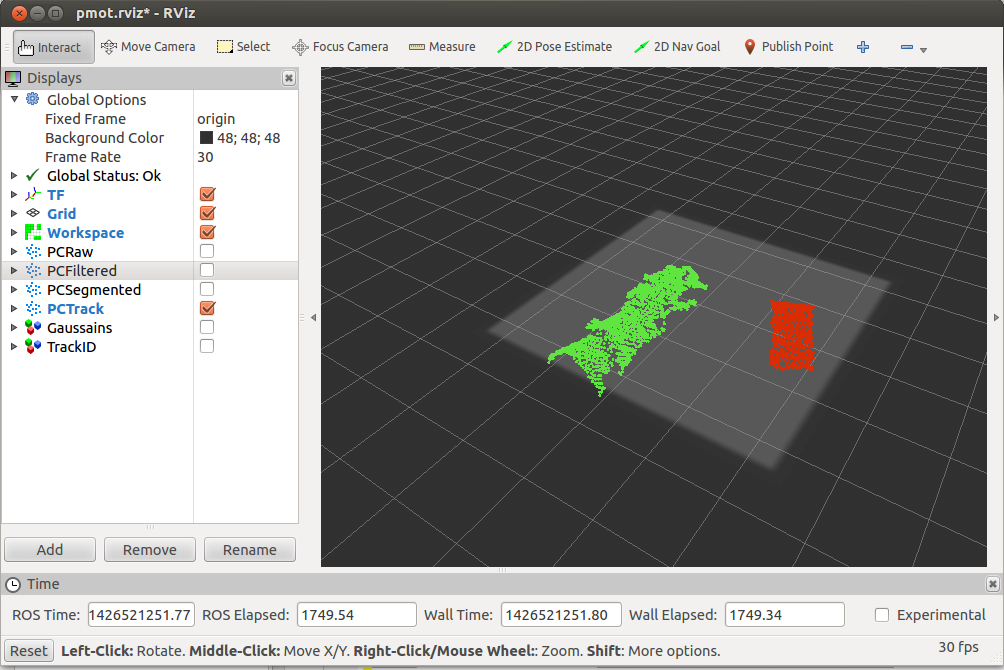
\includegraphics[width=0.45\linewidth]{fig/pmot_track_separated.png}%
		\label{fig:pmot_track_separated}}
	\hfil
	\subfloat[The contact case]{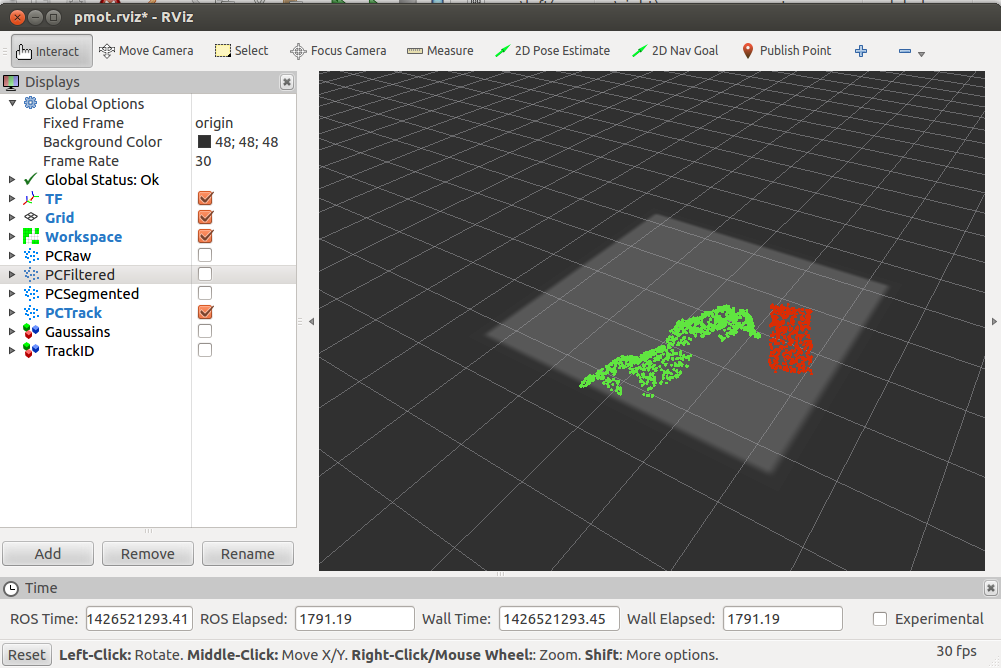
\includegraphics[width=0.45\linewidth]{fig/pmot_track_merged.png}%
		\label{fig:pmot_track_merged}}
	\caption{Existing point-cloud object tracking softwares}
	\label{fig:pmot_track}
\end{figure}

%_____Abbildungsverzeichnis_________________________________
\cleardoublepage
\addcontentsline{toc}{chapter}{List of Figures} 
\listoffigures 	 %Abbildungsverzeichnis

%___________________________________________________________

%_____Literaturverzeichnis_________________________________
\cleardoublepage
\addcontentsline{toc}{chapter}{Bibliography}
\bibliography{bib}
\bibliographystyle{alphaurl}
%__________________________________________________________


%_____License_________________________________
%\cleardoublepage
%\chapter*{License}
%\markright{LICENSE}
%This work is licensed under the Creative Commons Attribution 3.0 Germany
%License. To view a copy of this license,
%visit %\href{http://creativecommons.org/licenses/by/3.0/de/}{http://creativecommons.org} or send a letter
%to Creative Commons, 171 Second Street, Suite 300, San
%Francisco, California 94105, USA.
%__________________________________________________________

\end{document}
